% !TeX program = xelatex
\documentclass[UTF8,a4paper,11pt,fontset=windows]{ctexart}
\usepackage[margin=22mm]{geometry}
\usepackage{amsmath,amssymb,bm,booktabs,longtable,array,graphicx,float}
\usepackage{pdflscape,tikz,listings,xcolor}
\usetikzlibrary{arrows.meta,positioning,calc}
\usepackage[colorlinks=true,linkcolor=blue!55!black,urlcolor=blue!55!black]{hyperref}
\setcounter{tocdepth}{2}
\setcounter{MaxMatrixCols}{12}
\setlength{\parskip}{0.35em}
\setlength{\emergencystretch}{2em}
\renewcommand{\arraystretch}{1.15}
\lstset{language=Matlab,basicstyle=\ttfamily\small,breaklines=true,
  columns=fullflexible,frame=single,showstringspaces=false,
  keywordstyle=\color{blue!60!black},commentstyle=\color{green!35!black}}
\newcommand{\dd}{\mathrm{d}}
\newcommand{\de}{\delta_e}
\newcommand{\dt}{\delta_T}
\newcommand{\Gq}{G_{q\delta_e}}
\newcommand{\file}[1]{\mbox{\texttt{\small\detokenize{#1}}}}
\title{AERO5560 Group 8\\飞机建模与俯仰角速度反馈回路\\\large 阶段报告：数据、配平、线性化与内环设计}
\author{Group 8}
\date{2026年10月20日}
\begin{document}
\maketitle
\begin{abstract}
本报告给出 Group 8 飞机数据、配平检查、数值 $A/B$ 矩阵、$G_{q\delta_e}$ 与三轮内环设计。所选闭环带宽为 4.237 rad/s，调节时间 1.607 s，稳态误差 0.116\%，超调 8.897\%；20 rad/s 开环与闭环噪声幅值分别为 -41.390、-41.409 dB。名义指标达标，并完成非名义与非线性验证。
\end{abstract}
\clearpage
\tableofcontents
\clearpage

\section{任务范围与建模约定}
本报告完成纵向 Task 1 的飞机建模、$\Gq$ 提取、反馈框图与三轮补偿器设计。后续工作包括垂直速度外环、阵风分析、自动油门与完整系统集成。

采用机体系速度与角速度、Euler 姿态角及地面位置状态：
\begin{equation}
\bm X=[u,v,w,p,q,r,\phi,\theta,\psi,X_e,Y_e,Z_e]^{\mathsf T}.
\end{equation}
操纵输入为
\begin{equation}
\bm U=[\dt,\de,\delta_a,\delta_r,\delta_f]^{\mathsf T},
\end{equation}
分别表示油门、升降舵、副翼、方向舵和襟翼。内部使用 SI 单位：速度 m/s、位置 m、角度 rad、角速度 rad/s，油门为 $0$--$1$ 比例。地面高度 $h=-Z_e$，垂直速度 $V_s=-\dot Z_e$，向上为正。

线性模型中的变量均为相对标称飞行轨迹的增量：
\begin{equation}
\bm X=\bm X_{\rm ref}(t)+\Delta\bm X,\qquad
\bm U=\bm U_0+\Delta\bm U.
\end{equation}
参考轨迹沿 $X_e$ 方向前进，操纵变量采用相对 $\bm U_0$ 的增量。

\section{Group 8 飞机数据}
通过 MATLAB R2025b Update 7 执行本组 \file{FlightDataAircraft8.p}。初始条件加载自 \file{ICsAircraft8_200knts_300ft.mat}。

\subsection{质量、几何与推进参数}
\begin{table}[H]\centering
\caption{读取的主要飞机参数}
\begin{tabular}{llr}\toprule
参数&含义&数值\\\midrule
$m$&质量&750 kg\\
$g$&重力加速度&9.81 m/s$^2$\\
$S$&参考翼面积&11.9 m$^2$\\
$b$&翼展&7 m\\
$c$&参考弦长&0.85 m\\
$I_{xx}$&滚转惯量&605.29 kg\,m$^2$\\
$I_{yy}$&俯仰惯量&1766.52 kg\,m$^2$\\
$I_{zz}$&偏航惯量&2168.83 kg\,m$^2$\\
$I_{xz}$&惯性积参数&84.71 kg\,m$^2$\\
$P_{\max}$&最大功率参数&253.504 kW\\
$\eta$&螺旋桨效率参数&0.85\\\bottomrule
\end{tabular}
\end{table}
由参数可得展弦比 $b^2/S=4.11765$，翼载 $mg/S=618.277\,\mathrm{N/m^2}$。

为兼容当前课程非线性框架，按数据包说明添加旧字段的映射：
\begin{lstlisting}
FlightData = FlightDataAircraft8();
FlightData.Geometric = FlightData.Geo;
FlightData.Inertial = FlightData.I;
FlightData.Propeller = FlightData.Prop;
\end{lstlisting}
\subsection{初始状态与操纵量}
\begin{equation}
\begin{aligned}
\bm X_0={}&[102.8869153573,\;0,\;0.4724322704,\;0,\;0,\;0,\\
 &\phantom{[}0,\;0.004591730139,\;0,\;0,\;0,\;-91.44]^{\mathsf T},
\end{aligned}
\end{equation}
\begin{equation}
\bm U_0=[0.7703166691,\;0.01337052176,\;0,\;0,\;0]^{\mathsf T}.
\end{equation}
飞行条件见表~\ref{tab:trimpoint}。
\begin{table}[H]\centering
\caption{初始飞行条件与操纵量}\label{tab:trimpoint}
\begin{tabular}{lr}\toprule
项目&数值\\\midrule
$V_0=\sqrt{u_0^2+v_0^2+w_0^2}$&102.888 m/s，约 199.99827 knots\\
$h_0=-Z_{e0}$&91.44 m，300 ft\\
$\alpha_0=\operatorname{atan2}(w_0,u_0)$&$0.263086758^\circ$\\
$\theta_0$&$0.263086758^\circ$\\
$\beta_0,\phi_0,\psi_0$&$0$\\
$p_0,q_0,r_0$&$0$\\
油门&$77.0316669\%$\\
升降舵&$+0.766074467^\circ$\\
副翼、方向舵、襟翼&$0^\circ$\\\bottomrule
\end{tabular}
\end{table}

地面垂直速度为
\begin{equation}\label{eq:vs}
V_s=u\sin\theta-v\sin\phi\cos\theta-w\cos\phi\cos\theta.
\end{equation}
代入本组初值得到 $V_{s0}=0$，与 $\theta_0=\alpha_0$ 的水平飞行条件一致。

\subsection{操纵限位}
本组数据给定油门范围 $[0,1]$，升降舵、副翼和方向舵均为 $\pm25^\circ$。任务书对副翼明确要求 $\pm20^\circ$，后续横向验收采用更严格的任务书限制。数据没有给出襟翼限位或舵速限制。

对俯仰内环，必须检查绝对升降舵：
\begin{equation}\label{eq:limit}
-25^\circ\leq\delta_{e0}+\Delta\de(t)\leq25^\circ.
\end{equation}
因 $\delta_{e0}=0.766074467^\circ$，可用的增量范围约为
$[-25.766074467^\circ,\;24.233925533^\circ]$。油门正向增量余量为 $1-0.7703166691=0.2296833309$。

\section{非线性配平检查}
\subsection{方法}
使用零阵风、原始 $\bm X_0,\bm U_0$，调用 \file{aero5560_aero.p} 与 \file{aero5560_motion.p}。气动函数依赖状态导数，因此需要一致性迭代：
\begin{align}
(\bm C_F^{(k)},\bm C_M^{(k)})
 &=\mathcal A(\bm X_0,\bm 0,\dot{\bm X}^{(k)},\bm U_0,F),\\
\dot{\bm X}^{(k+1)}
 &=\mathcal M(\bm X_0,\bm C_F^{(k)},\bm C_M^{(k)},F).
\end{align}
以相邻迭代差的无穷范数小于 $10^{-11}$ 为终止条件，并设置最大迭代次数。当前初始点迭代两次收敛，最后更新范数为零。

\subsection{残差与自由运行结果}
\begin{table}[H]\centering
\caption{初始状态导数检查}
\begin{tabular}{ll}\toprule
项目&结果\\\midrule
$\dot u$&$-2.4980\times10^{-16}$ m/s$^2$\\
$\dot v,\dot w$&$0$ m/s$^2$\\
$\dot p,\dot q,\dot r$&$0$ rad/s$^2$\\
$\dot\phi,\dot\theta,\dot\psi$&$0$ rad/s\\
$\dot X_e$&$102.888$ m/s，正常前进\\
$\dot Y_e,\dot Z_e$&$0$ m/s\\\bottomrule
\end{tabular}
\end{table}
本次工程诊断容差为：平动加速度 $10^{-4}$ m/s$^2$、角加速度和姿态变化率 $10^{-6}$（各自 SI 单位）、侧向及垂向地面速度 $10^{-4}$ m/s。

固定 $\bm U_0$、不加入阵风与反馈，使用 \texttt{ode45} 积分 60 s。第一组设置为相对容差 $10^{-9}$、绝对容差 $10^{-11}$、最大步长 0.05 s；复核组为 $10^{-10}$、$10^{-12}$、0.025 s。输出采样间隔为 0.1 s，共 601 点。

两组计算的速度、高度、垂直速度、迎角、俯仰角及三轴角速度均保持初值，输出差异在保存的双精度数值中为零。$X_e(60)\approx6173.28$ m，与 $V_0t$ 一致。可保留给定配平点用于线性化。图~\ref{fig:trim} 给出实际计算图。
\begin{figure}[H]\centering
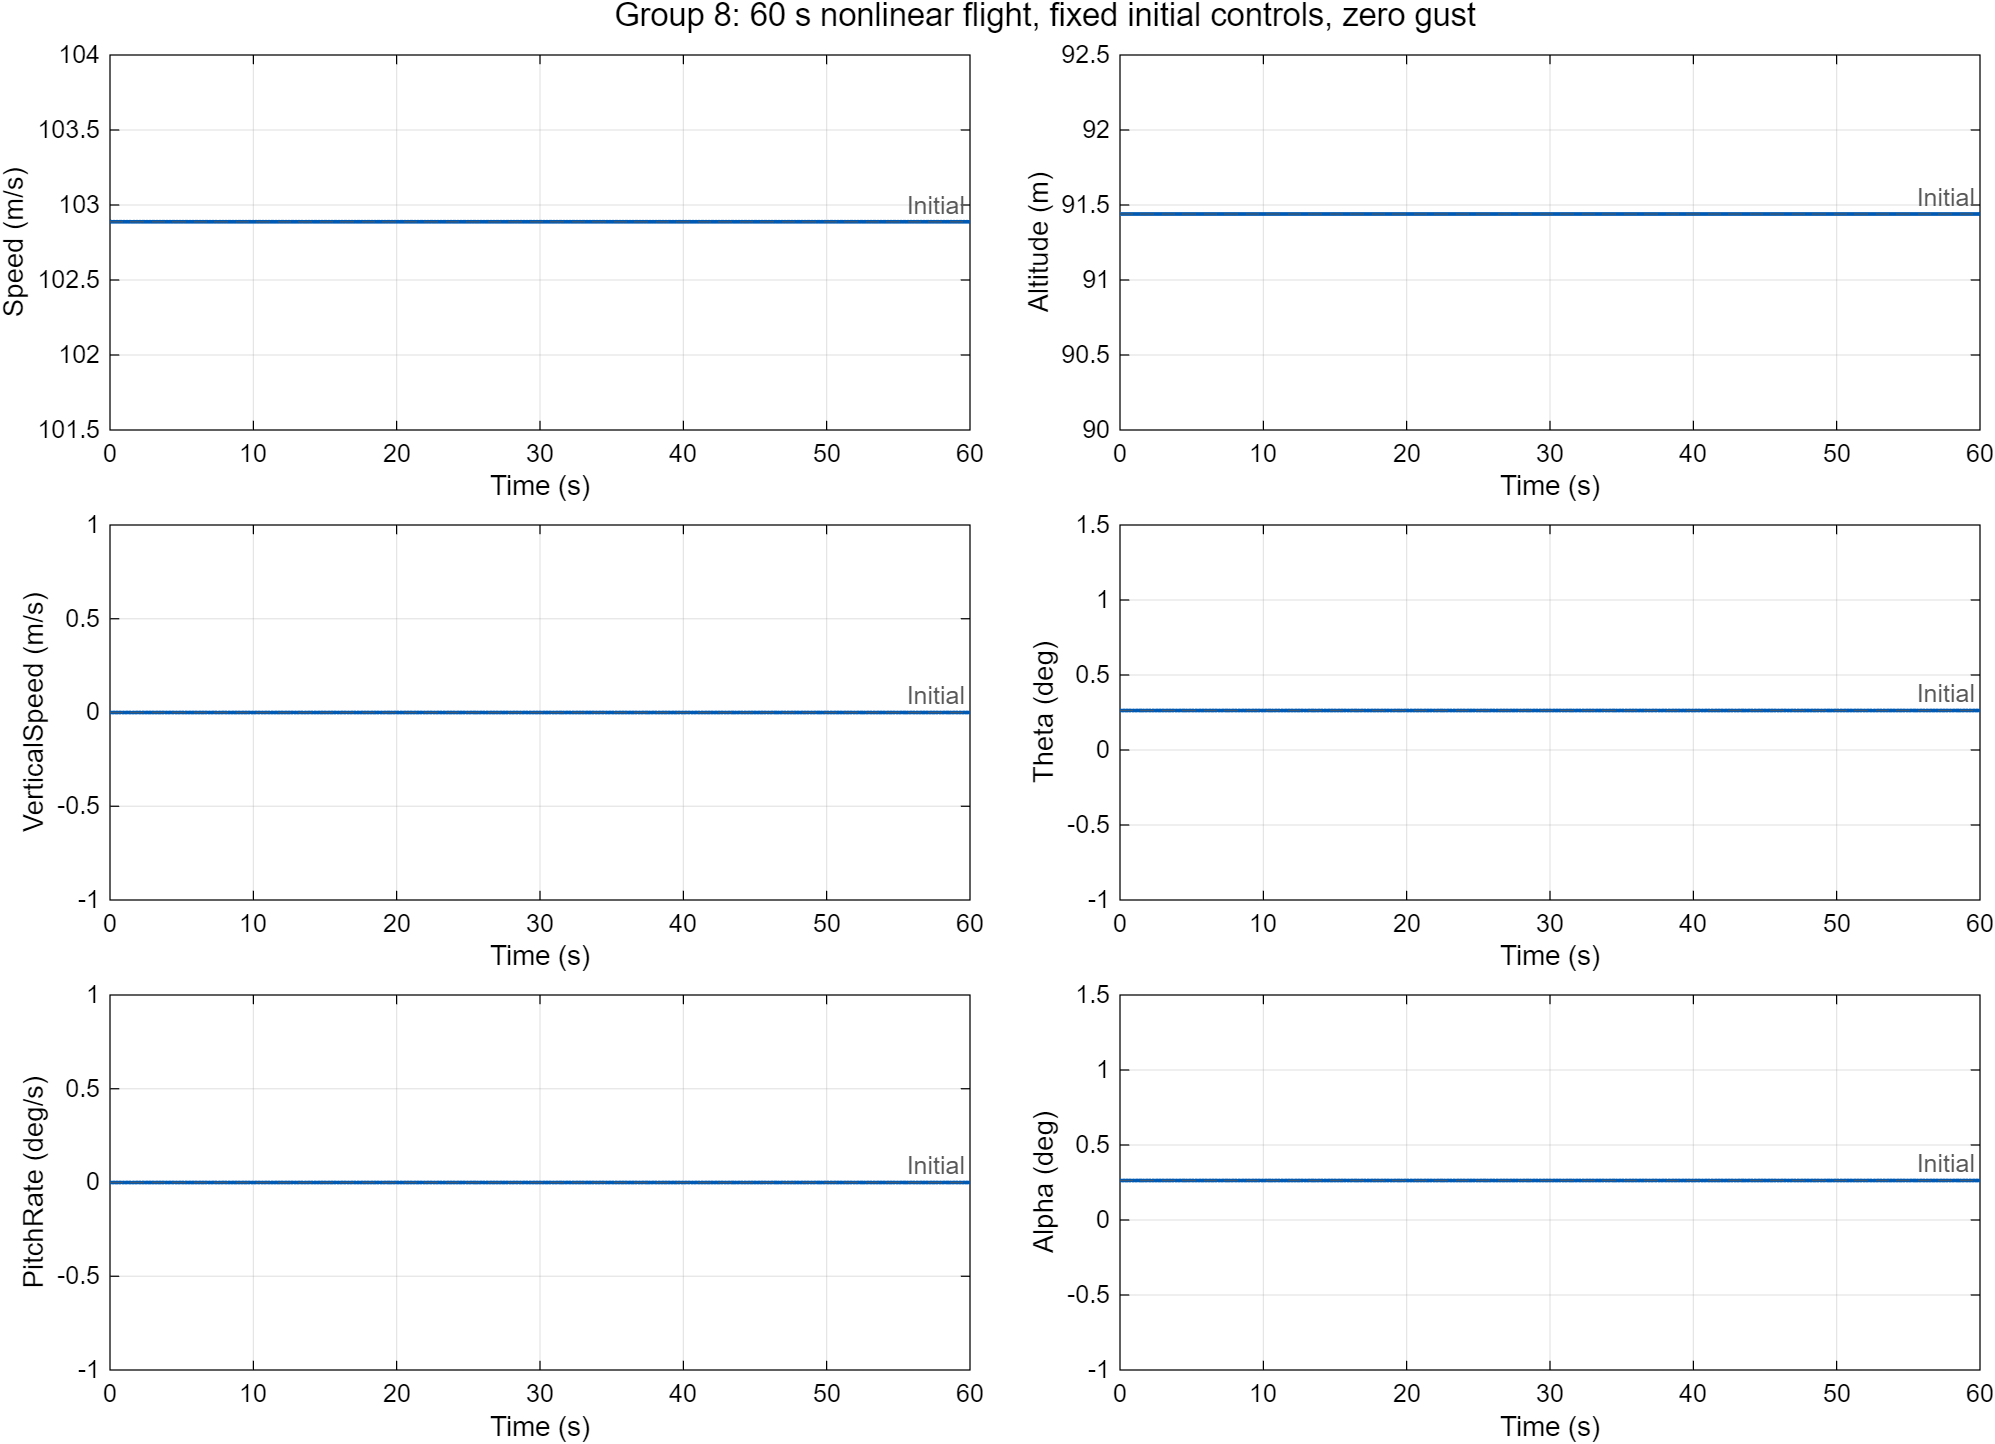
\includegraphics[width=0.94\linewidth]{trim.png}
\caption{Group 8 在固定初始操纵量、零阵风条件下的 60 s 非线性自由运行。}\label{fig:trim}
\end{figure}
稳定性由下文线性化极点与扰动响应评价。

\section{数值线性化与状态空间模型}
\subsection{中心差分与数值验证}
在配平轨迹附近写为
\begin{equation}\label{eq:ss}
\Delta\dot{\bm X}=A\Delta\bm X+B\Delta\bm U.
\end{equation}
逐列使用中心差分：
\begin{align}
A_{:,i}&\approx\frac{f(\bm X_0+h_i\bm e_i,\bm U_0)-f(\bm X_0-h_i\bm e_i,\bm U_0)}{2h_i},\\
B_{:,j}&\approx\frac{f(\bm X_0,\bm U_0+k_j\bm e_j)-f(\bm X_0,\bm U_0-k_j\bm e_j)}{2k_j}.
\end{align}
每次求 $f$ 都重新迭代隐式状态导数。状态扰动按速度、角度/角速度及位置的尺度设置，输入尺度取 1；比较相对步长 $10^{-4},3\times10^{-5},10^{-5},3\times10^{-6},10^{-6}$，选用中间的 $10^{-5}$。

\begin{table}[H]\centering
\caption{相对所选差分结果的整体 Frobenius 范数差}
\begin{tabular}{rrr}\toprule
相对步长&$\|A_h-A\|_F/\|A\|_F$&$\|B_h-B\|_F/\|B\|_F$\\\midrule
$10^{-4}$&$1.1803\times10^{-9}$&$5.1592\times10^{-12}$\\
$3\times10^{-5}$&$9.5524\times10^{-11}$&$5.5809\times10^{-13}$\\
$10^{-5}$&$0$&$0$\\
$3\times10^{-6}$&$1.1302\times10^{-11}$&$1.6652\times10^{-11}$\\
$10^{-6}$&$2.3360\times10^{-10}$&$9.7214\times10^{-11}$\\\bottomrule
\end{tabular}
\end{table}
用独立混合扰动检查 Taylor 余项；扰动幅度连续减半时，余项由约 $5.2498\times10^{-5}$、$1.3124\times10^{-5}$ 减为 $3.2808\times10^{-6}$，缩小比为 4.0002、4.0001，符合一阶线性化的二阶余项特性。

\subsection{纵向四状态模型}
固定高度近似下，取状态索引 $[1,3,5,8]$、输入索引 $[1,2]$：
\begin{equation}
\bm x_\ell=[\Delta u,\Delta w,\Delta q,\Delta\theta]^{\mathsf T},\qquad
\bm u_\ell=[\Delta\dt,\Delta\de]^{\mathsf T}.
\end{equation}
\begin{equation}\label{eq:alon}
A_\ell=\begin{bmatrix}
-0.06144334&0.05552868&-0.47243227&-9.80989658\\
-0.16960655&-4.78731236&99.44823052&-0.04504471\\
0.0002475794&-0.11258862&-3.67476184&0\\
0&0&1&0
\end{bmatrix},
\end{equation}
\begin{equation}\label{eq:blon}
B_\ell=\begin{bmatrix}
2.76318036&0\\
-5.9699623\times10^{-5}&-62.90658081\\
-1.7950804\times10^{-5}&-88.19693912\\
0&0
\end{bmatrix}.
\end{equation}
第二个状态为机体系速度 $w$。

纵向四状态特征值为
\begin{equation}
\lambda_{\rm SP}=-4.2313617\pm3.3004001\mathrm i,\qquad
\lambda_{\rm ph}=-0.03039711\pm0.07729208\mathrm i.
\end{equation}
分别对应短周期和长周期，均位于左半平面。

\subsection{高度状态及横航向模型}
完整 $A$ 的 $Z_e$ 列存在非零项；含高度的纵向状态可取 $[u,w,q,\theta,Z_e]$，其矩阵已保存。四状态近似忽略高度反馈，本报告提取 $\Gq$ 使用式~\eqref{eq:alon}--\eqref{eq:blon}。

横航向状态取 $[v,p,r,\phi,\psi]$，输入为副翼和方向舵。其极点约为 $-13.81679$、$-0.719193\pm2.625197\mathrm i$、$-0.0119723$ 及航向积分极点 0。位置与航向包含中性运动学模态。完整矩阵及附加子矩阵见附录。

\subsection{小阶跃线性与非线性比较}
采用完整 12 状态 $A,B$，分别施加 $+0.05^\circ$ 升降舵增量和 $+0.001$ 油门增量，仿真 10 s。线性解使用矩阵指数，非线性解使用 \texttt{ode45}；比较速度、$q$ 与由式~\eqref{eq:vs} 定义的垂直速度。
\begin{table}[H]\centering
\caption{10 s 比较中的输出最大绝对误差}
\begin{tabular}{lrrr}\toprule
测试&速度 (m/s)&$q$ ($^\circ$/s)&$V_s$ (m/s)\\\midrule
升降舵增量&0.016588&0.023974&0.641690\\
油门增量&$2.0867\times10^{-6}$&$1.3892\times10^{-7}$&$2.5237\times10^{-7}$\\\bottomrule
\end{tabular}
\end{table}
升降舵测试前 2 s 的 $V_s$ 最大误差约 0.004968 m/s，为同期非线性响应峰值的 0.2253\%。但到 10 s，$V_s$ 峰值约 11.93 m/s、速度变化约 4.69 m/s，已逐渐偏离初始点，$V_s$ 相对误差升至约 5.38\%。误差随飞机偏离配平点而增大。

\section{提取升降舵到俯仰角速度的传递函数}
\subsection{输出选择与推导}
纵向输入的第二列为升降舵。令
\begin{equation}
\begin{aligned}
B_q&=B_\ell(:,2)=\begin{bmatrix}0&-62.90658081&-88.19693912&0\end{bmatrix}^{\mathsf T},\\
C_q&=\begin{bmatrix}0&0&1&0\end{bmatrix},\qquad D_q=0.
\end{aligned}
\end{equation}
在零初始增量条件下进行 Laplace 变换：
\begin{align}
s\Delta\bm x_\ell&=A_\ell\Delta\bm x_\ell+B_q\Delta\de,\\
\Delta q&=C_q\Delta\bm x_\ell,
\end{align}
因此
\begin{equation}\label{eq:gdefinition}
\boxed{\Gq(s)=\frac{\Delta q(s)}{\Delta\de(s)}=C_q(sI-A_\ell)^{-1}B_q.}
\end{equation}
这里 $C_q$ 是状态空间输出矩阵，后文的互补灵敏度采用 $\mathcal C_q$ 表示，避免混淆。

\subsection{ZPK 与多项式表达}
ZPK 的实系数因式形式为
\begin{equation}\label{eq:gfactored}
\boxed{\Gq(s)=\frac{-88.19693912\,s(s+4.704978073)(s+0.06347365466)}
{(s^2+8.462723331s+28.79706207)(s^2+0.06079421306s+0.006898050455)}.}
\end{equation}
对应多项式形式为
\begin{equation}
\Gq(s)=\frac{-88.19693912s^3-420.5628467s^2-26.33932382s}
{s^4+8.523517544s^3+29.31844472s^2+1.809071019s+0.1986435871}.
\end{equation}
零点为
\begin{equation}
z=0,\quad -4.704978073,\quad -0.06347365466.
\end{equation}
极点为前述纵向四状态特征值，ZPK 增益为 $-88.19693912$。

\subsection{数值核对及物理解释}
在 $10^{-4}$ 至 $10^4$ rad/s 的 501 个频率点，将式~\eqref{eq:gfactored} 与状态空间频响比较，最大相对误差约为 $1.78\times10^{-13}$。另由 Cayley--Hamilton/Markov 递推独立形成多项式，频响最大相对误差约 $7.20\times10^{-9}$。

原始数值零点之一约为 $+2.40\times10^{-16}$。因当前模型满足 $q=\dot\theta$、$B_q$ 第四行为零且 $A_\ell$ 可逆，应有精确原点零点。程序核对该结构和 DC 增益后，将此浮点残差归零；保留原始对象，未进行一般零极点消去。

本模型 $\Gq(0)=0$：稳定开环飞机在恒定升降舵输入后，$q$ 最终回到零。高频首项约为 $-88.19694/s$，表示正升降舵增量对俯仰角加速度的直接作用为负。该符号在闭环设计中必须明确处理。

\section{俯仰角速度反馈回路构建}\label{sec:loop}
\subsection{控制目标与回路假设}
内环目标是利用升降舵，使实际俯仰角速度增量 $\Delta q$ 跟随指令 $\Delta q_c$。采用单位测量 $H_q(s)=1$、理想执行器 $A_e(s)=1$，并以线性小扰动模型设计。真实舵面限幅将在响应检查与非线性实现中按式~\eqref{eq:limit} 处理。

反馈结构采用有符号补偿器 $K_q(s)$。

\begin{figure}[H]\centering
\begin{tikzpicture}[>=Latex,font=\small,
  block/.style={draw,thick,minimum height=1.1cm,align=center,fill=blue!4},
  every path/.style={thick}]
\node[circle,draw,minimum size=0.7cm,inner sep=0pt] (sum) at (1.2,0) {};
\node at ($(sum.center)+(-0.15,0.12)$) {$+$};
\node at ($(sum.center)+(0.13,-0.15)$) {$-$};
\node[block,minimum width=2.8cm] (K) at (4.2,0) {补偿器\\$K_q(s)=-\bar K_q(s)$};
\node[block,minimum width=1.9cm] (act) at (8.0,0) {理想执行器\\$A_e(s)=1$};
\node[block,minimum width=2.3cm] (plant) at (11.6,0) {Group 8 飞机\\$\Gq(s)$};
\coordinate (take) at (13.3,0);
\node[block,minimum width=2.5cm] (sensor) at (8.0,-2.05) {理想角速度测量\\$H_q(s)=1$};
\draw[->] (-0.2,0) -- node[above] {$\Delta q_c(s)$} (sum.west);
\draw[->] (sum.east) -- node[above] {$e_q(s)$} (K.west);
\draw[->] (K.east) -- node[above] {$\Delta\delta_{e,c}(s)$} (act.west);
\draw[->] (act.east) -- node[above] {$\Delta\de(s)$} (plant.west);
\draw[->] (plant.east) -- (take) -- node[above] {$\Delta q(s)$} (14.6,0);
\fill (take) circle (1.6pt);
\draw[->] (take) |- (sensor.east);
\draw[->] (sensor.west) -| node[pos=0.18,above] {$\Delta q_m(s)$} (sum.south);
\node[align=center,font=\footnotesize] at (7.2,-3.05)
{角速度信号：rad/s；升降舵信号：rad；全部为相对配平的增量。};
\end{tikzpicture}
\caption{以升降舵控制俯仰角速度的单位负反馈回路。补偿器包含所需符号，最终参数见下文。}\label{fig:loop}
\end{figure}

\begin{table}[H]\centering
\caption{反馈框图中各信号与方块的定义}
\begin{tabular}{p{0.22\linewidth}p{0.56\linewidth}l}\toprule
标注&含义&单位\\\midrule
$\Delta q_c$&指令俯仰角速度增量&rad/s\\
$\Delta q_m$&测量反馈值，理想测量时等于 $\Delta q$&rad/s\\
$e_q$&指令减测量的误差&rad/s\\
$K_q(s)$&将角速度误差转换为升降舵指令的有符号补偿器&s\\
$\Delta\delta_{e,c}$&控制器给出的升降舵增量指令&rad\\
$A_e(s)=1$&理想执行器，实际增量等于指令增量&无量纲\\
$\Delta\de$&进入飞机模型的实际升降舵增量&rad\\
$\Gq(s)$&升降舵增量到 $q$ 的飞机开环动力学&$(\mathrm{rad/s})/\mathrm{rad}$\\
$\Delta q$&实际俯仰角速度增量&rad/s\\
$H_q(s)=1$&单位角速度测量反馈&无量纲\\\bottomrule
\end{tabular}
\end{table}

\subsection{反馈符号与工作过程}
比较点使用
\begin{equation}\label{eq:error}
e_q=\Delta q_c-\Delta q_m.
\end{equation}
飞机增益为负，正角速度误差需要负升降舵动作。符号包含在 $K_q=-\bar K_q$ 中，稳定性由极点与裕度检查。

信号关系依次为
\begin{align}
\Delta\delta_{e,c}&=K_q e_q,\\
\Delta\de&=A_e\Delta\delta_{e,c},\\
\Delta q&=\Gq\Delta\de,\\
\Delta q_m&=H_q\Delta q.
\end{align}
例如 $4^\circ$/s 指令对应 $\Delta q_c=4\pi/180\approx0.06981317$ rad/s。比较器、控制器与飞机内部均采用 rad 制，以免产生 $180/\pi$ 的比例错误。

\subsection{闭环推导与 SCK 表达式}
定义有符号环路传递函数
\begin{equation}
L_q=K_q A_e\Gq H_q.
\end{equation}
从式~\eqref{eq:error} 及前向关系可得
\begin{equation}
\Delta q=\Gq A_eK_q(\Delta q_c-H_q\Delta q),
\end{equation}
因此一般形式为
\begin{equation}
\frac{\Delta q}{\Delta q_c}=\frac{\Gq A_eK_q}{1+L_q},\qquad
\frac{\Delta\de}{\Delta q_c}=\frac{A_eK_q}{1+L_q}.
\end{equation}
在本节 $A_e=H_q=1$ 的假设下，定义灵敏度与互补灵敏度：
\begin{equation}\label{eq:sck}
S_q=\frac{1}{1+\Gq K_q},\qquad
\mathcal C_q=\frac{\Gq K_q}{1+\Gq K_q},\qquad S_q+\mathcal C_q=1.
\end{equation}
于是有
\begin{equation}\label{eq:cl}
\boxed{\frac{\Delta q}{\Delta q_c}=\mathcal C_q,\quad
\frac{e_q}{\Delta q_c}=S_q,\quad
\frac{\Delta\de}{\Delta q_c}=K_qS_q.}
\end{equation}
其中 $\mathcal C_q$ 用于指令跟踪，$S_q$ 用于误差与适当扰动入口的分析，$K_qS_q$ 用于升降舵需求检查。这里没有预先将噪声或阵风注入未标注的位置；后续阵风传递函数需按实际入口重新推导。

令式~\eqref{eq:gfactored} 的分子、分母为 $N_G,D_G$，且 $K_q=N_K/D_K$，则闭环特征方程为
\begin{equation}
D_GD_K+N_GN_K=0.
\end{equation}
该式中的 $N_K$ 包含控制器符号，最终数值 ZPK 见 \file{inner_loop/zpk.txt}。

\subsection{实际输入偏置与 MATLAB 构造}
线性回路输出的是 $\Delta\de$。进入非线性飞机时需执行
\begin{equation}
\de(t)=0.01337052176+\Delta\de(t)\quad(\mathrm{rad}),
\end{equation}
并在非线性实现中执行绝对舵角限幅。

对本次选定的有符号 $K_q$，可在 MATLAB 构造同一回路：
\begin{lstlisting}
load('Gqde.mat', 'Gqde');
Lq = Gqde * Kq;
Sq = feedback(1, Lq);       % error / q_command
Cq_closed = feedback(Lq,1); % q / q_command
Uq = feedback(Kq,Gqde);     % elevator_increment / q_command
\end{lstlisting}
\file{loop.m} 根据传入的有符号 $K_q$ 构造反馈模型。

\clearpage\section{俯仰角速度内环设计}
200 节、300 ft 时，所选闭环带宽为 4.237 rad/s，开环交越频率为 2.017 rad/s；短周期固有频率为 5.366 rad/s。三轮补偿器为：
\begin{align}
K_{q,1}(s)&=-0.1961/s,\\
K_{q,2}(s)&=\frac{-5.835(s+0.5)}{s(s+0.1)(s+30)},\\
K_{q,3}(s)&=\frac{-21.5(s+0.136)(s+0.16)}{s(s+0.0015)(s+0.31)(s+10.7)(s+14.5)}.
\end{align}
SISOtool 使用 $P_q=\operatorname{minreal}(-G/s)$ 与 $F_q=-sK_q$。一个积分器抵消最小 q 通道的原点零点；所得 type-0 开环需满足 $L(0)>99$，使误差小于 1\%。控制器零极点均为实数，开环严格真有理。
\begin{table}[H]\centering\small\caption{三轮补偿器指标}
\begin{tabular}{lrrr}\toprule
指标 & 1 & 2 & 3\\\midrule
$t_s$ (s) & 10.919 & 4.546 & 1.607\\
$t_{s,command}$ (s) & $\infty$ & 3.938 & 1.602\\
SSE (\%) & 3.703 & 0.770 & 0.116\\
Overshoot (\%) & 3.516 & 16.787 & 8.897\\
$\omega_{BW}$ (rad/s) & 5.211 & 5.645 & 4.237\\
$|L(j20)|$ (dB) & -27.220 & -28.885 & -41.390\\
$|T(j20)|$ (dB) & -26.841 & -28.595 & -41.409\\
\bottomrule\end{tabular}\end{table}

4 deg/s 阶跃前 10 s 的绝对升降舵为 0.4194--0.7661 度，相位裕度 60.301 度，增益裕度 10.806 dB。20 rad/s 噪声幅值满足 Lecture 9-1 第 9、17 页的 $-40$ dB 标准，20--$10^5$ rad/s 检查频段也全部通过。

独立配平的 180、200、210 节工况满足主要时域和噪声指标。假设 50 ms 舵机的超调为 15.88\%，主要名义指标通过；100 ms 时超调 22.31\%、调节时间 3.757 s，两项超限。27 种参数扰动中，21 种满足全部时域阈值。

由 $\dot\theta=q$，未约简系统保留中性模态。2 s 非线性脉冲的载荷峰值为 1.759 g，固定油门时速度降至 93.874 m/s，后续仍需姿态管理与自动油门。
\begin{figure}[H]\centering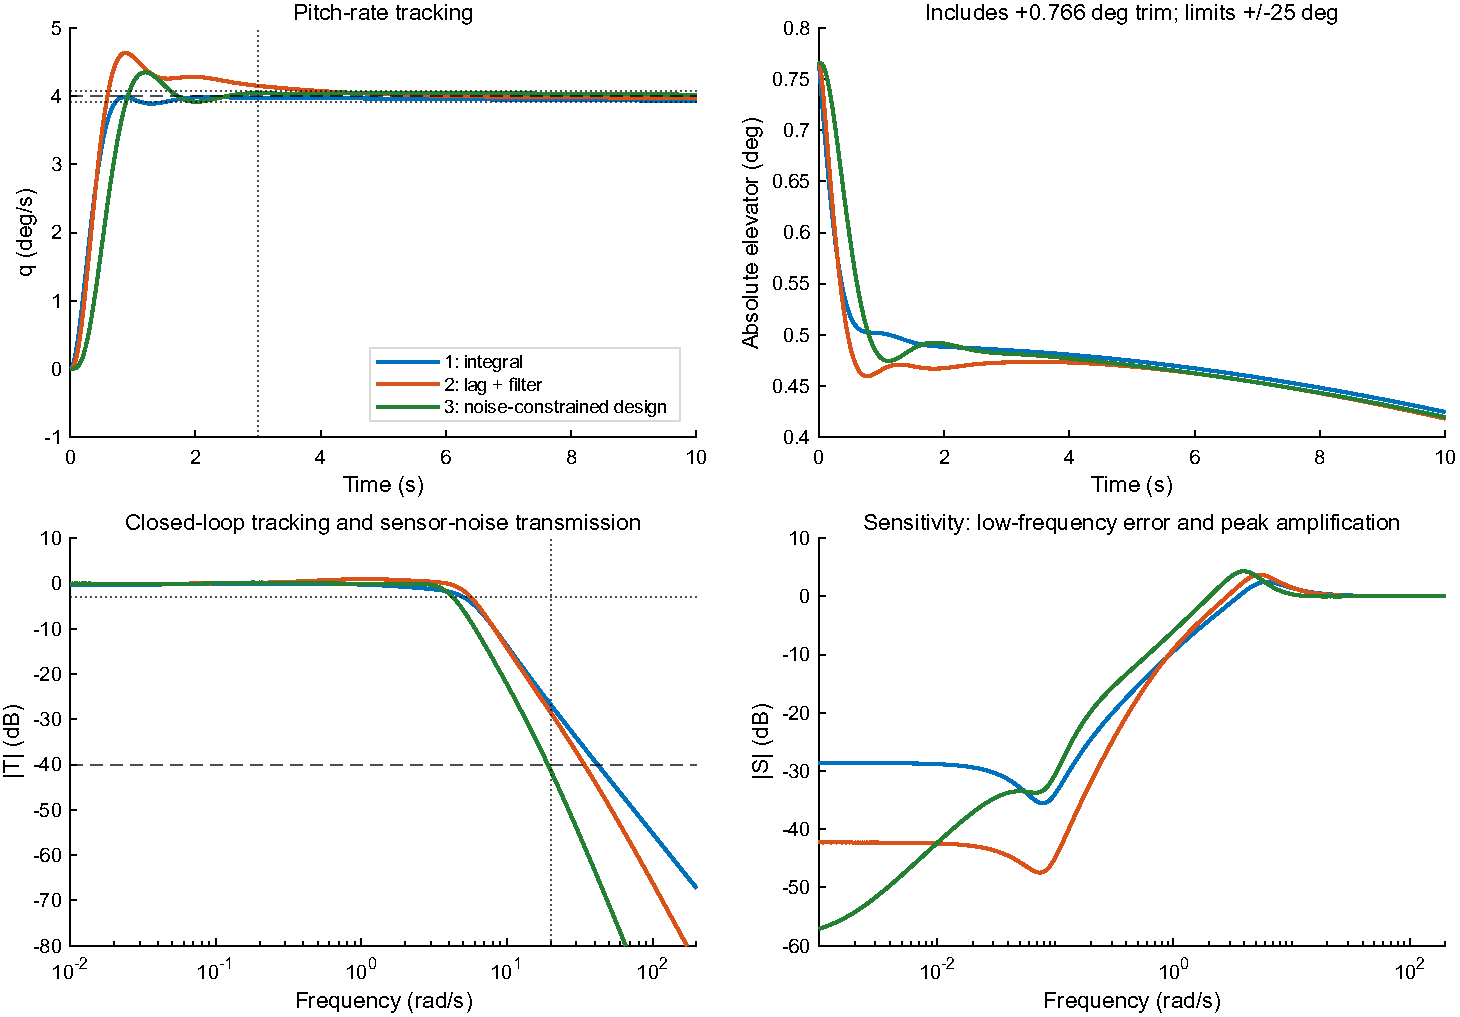
\includegraphics[width=\linewidth]{../inner_loop/comparison.pdf}
\caption{三轮设计的 q、升降舵、互补灵敏度与灵敏度。}\end{figure}
完整图表与验证见\href{../inner_loop/inner_loop_report.pdf}{详细内环报告}。运行 \file{inner_loop/run_inner.m} 复现，使用 \file{open_sisotool(3)} 查看模型。

\section{文件、复现与来源}
\begin{table}[H]\centering
\caption{当前项目中的计算文件与结果}
\begin{tabular}{p{0.47\linewidth}p{0.43\linewidth}}\toprule
目录/入口&用途\\\midrule
\file{trim/run_trim.m}&配平残差、60 s 自由运行及积分复核\\
\file{A_B_Matrix/run_linear.m}&中心差分 A/B、子系统、特征值及局部验证\\
\file{Gqde/run_Gqde.m}&提取本组 $\Gq$ 并核对频响\\
\file{AI_draft/loop.m}&传入有符号补偿器后构造本节反馈传递关系\\
\file{AI_draft/report.tex}&本单一 LaTeX 源文件，框图使用原生 TikZ\\
\file{AI_draft/trim.png}&由实际配平仿真导出的图\\\bottomrule
\end{tabular}
\end{table}
本报告打印矩阵与系数经过舍入，后续计算应读取 MAT/JSON 中的完整精度数值。

\begin{thebibliography}{9}
\bibitem{brief} AERO5560, \emph{Group Project: Aircraft Closed-Loop Control System Design and Analysis}, 项目任务书，第 1--5 页。
\bibitem{data} \emph{Group8 AircraftData}: \file{FlightDataAircraft8.p}、\file{ICsAircraft8_200knts_300ft.mat} 与 \file{Note.txt}。
\bibitem{framework} AERO5560, \emph{Flight Simulation Student Version}, 课程非线性函数及接口说明。
\bibitem{lectures} AERO5560, Lectures 1-2、2-1/2、7-2、8-1/2、9-1/2、10-1：线性化、传递函数、反馈结构及控制器设计。
\end{thebibliography}

\appendix
\clearpage
\begin{landscape}
\thispagestyle{plain}
\section{完整十二状态矩阵}
状态与输入顺序见正文第 1 节。下列矩阵保留约 8 位有效数字；每个元素的单位由对应状态导数单位与列变量单位之比确定。
\begin{center}\setlength{\arraycolsep}{3pt}\resizebox{\linewidth}{!}{$A=\begin{bmatrix}
-0.061443341 & 0 & 0.05552868 & 0 & -0.47243227 & 0 & 0 & -9.8098966 & 0 & 0 & 0 & 3.1754685\times10^{-5} \\
0 & -0.37729298 & 0 & 0.53108604 & 0 & -102.86881 & 9.8487485 & 0 & 0 & 0 & 0 & 0 \\
-0.16960655 & 0 & -4.7873124 & 0 & 99.448231 & 0 & 0 & -0.045044714 & 0 & 0 & 0 & -0.00094886847 \\
0 & -0.20268929 & 0 & -13.808594 & 0 & 1.4524332 & 0.019116101 & 0 & 0 & 0 & 0 & 0 \\
0.00024757942 & 0 & -0.11258862 & 0 & -3.6747618 & 0 & 0 & 0 & 0 & 0 & 0 & -1.3364074\times10^{-6} \\
0 & 0.058710969 & 0 & -0.54309133 & 0 & -1.0812624 & -0.0033528581 & 0 & 0 & 0 & 0 & 0 \\
0 & 0 & 0 & 1 & 0 & 0.0045917624 & 0 & 0 & 0 & 0 & 0 & 0 \\
0 & 0 & 0 & 0 & 1 & 0 & 0 & 0 & 0 & 0 & 0 & 0 \\
0 & 0 & 0 & 0 & 0 & 1.0000105 & 0 & 0 & 0 & 0 & 0 & 0 \\
0.99998946 & 0 & 0.004591714 & 0 & 0 & 0 & 0 & 0 & 0 & 0 & 0 & 0 \\
0 & 1 & 0 & 0 & 0 & 0 & -0.47243227 & 0 & 102.888 & 0 & 0 & 0 \\
-0.004591714 & 0 & 0.99998946 & 0 & 0 & 0 & 0 & -102.888 & 0 & 0 & 0 & 0 \\
\end{bmatrix}$}\end{center}
\end{landscape}
\clearpage
\subsection{完整输入矩阵}\begin{equation}B=\begin{bmatrix}
2.7631804 & 0 & 0 & 0 & 0 \\
0 & 0 & 3.7014393 & 20.777334 & 0 \\
-5.9699623\times10^{-5} & -62.906581 & 0 & 0 & 0 \\
0 & 0 & -318.33488 & -3.5101752 & 0 \\
-1.7950804\times10^{-5} & -88.196939 & 0 & 0 & 0 \\
0 & 0 & -16.168938 & -27.867108 & 0 \\
0 & 0 & 0 & 0 & 0 \\
0 & 0 & 0 & 0 & 0 \\
0 & 0 & 0 & 0 & 0 \\
0 & 0 & 0 & 0 & 0 \\
0 & 0 & 0 & 0 & 0 \\
0 & 0 & 0 & 0 & 0 \\
\end{bmatrix}\end{equation}

\section{附加子系统矩阵}
\subsection{含高度的纵向五状态模型}
状态 $[u,w,q,\theta,Z_e]$，输入 $[\dt,\de]$。
\begin{equation}\resizebox{0.95\linewidth}{!}{$A_{\ell,5}=\begin{bmatrix}
-0.061443341 & 0.05552868 & -0.47243227 & -9.8098966 & 3.1754685\times10^{-5} \\
-0.16960655 & -4.7873124 & 99.448231 & -0.045044714 & -0.00094886847 \\
0.00024757942 & -0.11258862 & -3.6747618 & 0 & -1.3364074\times10^{-6} \\
0 & 0 & 1 & 0 & 0 \\
-0.004591714 & 0.99998946 & 0 & -102.888 & 0 \\
\end{bmatrix}$}\end{equation}
\begin{equation}B_{\ell,5}=\begin{bmatrix}
2.7631804 & 0 \\
-5.9699623\times10^{-5} & -62.906581 \\
-1.7950804\times10^{-5} & -88.196939 \\
0 & 0 \\
0 & 0 \\
\end{bmatrix}\end{equation}
\subsection{横航向五状态模型}
状态 $[v,p,r,\phi,\psi]$，输入 $[\delta_a,\delta_r]$。
\begin{equation}\resizebox{0.95\linewidth}{!}{$A_{\rm lat}=\begin{bmatrix}
-0.37729298 & 0.53108604 & -102.86881 & 9.8487485 & 0 \\
-0.20268929 & -13.808594 & 1.4524332 & 0.019116101 & 0 \\
0.058710969 & -0.54309133 & -1.0812624 & -0.0033528581 & 0 \\
0 & 1 & 0.0045917624 & 0 & 0 \\
0 & 0 & 1.0000105 & 0 & 0 \\
\end{bmatrix}$}\end{equation}
\begin{equation}B_{\rm lat}=\begin{bmatrix}
3.7014393 & 20.777334 \\
-318.33488 & -3.5101752 \\
-16.168938 & -27.867108 \\
0 & 0 \\
0 & 0 \\
\end{bmatrix}\end{equation}

\clearpage
\section{读取的完整气动参数}
保留原始参数字段名。气动导数遵循原模型的无量纲约定，$A/B$ 通过数值线性化获得。
\begingroup\small\renewcommand{\arraystretch}{1.05}
\begin{table}[H]\centering\caption{Group 8 原始气动字段}\label{tab:aero}
\begin{tabular}{lrlr}\toprule 字段&数值&字段&数值\\\midrule
\file{alpha_o} & $-0.013772917$ & \file{Cmad} & $0.9531$ \\
\file{Cdo} & $0.020342$ & \file{Cmde} & $-2.3941614$ \\
\file{k} & $0.063776$ & \file{Cnb} & $0.027705$ \\
\file{CLa} & $4.786$ & \file{Cnbd} & $-0.0051$ \\
\file{CLq} & $9.269$ & \file{Cnp} & $-0.000421$ \\
\file{CLad} & $-1.1439$ & \file{Cnr} & $-0.140618$ \\
\file{CLde} & $0.61398157$ & \file{Cnda} & $-0.015126086$ \\
\file{CLo} & $0.065917179$ & \file{Cndr} & $-0.11229973$ \\
\file{Cyb} & $-0.379162$ & \file{Clb} & $-0.024446$ \\
\file{Cybd} & $0.117$ & \file{Clbd} & $0.0068$ \\
\file{Cyp} & $0.016304$ & \file{Clp} & $-0.456441$ \\
\file{Cyr} & $0.1222$ & \file{Clr} & $0.0601$ \\
\file{Cyda} & $0.036153637$ & \file{Clda} & $-0.35735378$ \\
\file{Cydr} & $0.20294165$ & \file{Cldr} & $0.000394$ \\
\file{Cmo} & $0.03337$ & \file{CDdf} & $0$ \\
\file{Cma} & $-0.295926$ & \file{CLdf} & $0$ \\
\file{Cmq} & $-25.094866$ & \file{Cmdf} & $0$ \\
\bottomrule\end{tabular}\end{table}\endgroup
\end{document}
